\documentclass{article}
\usepackage[a4paper, top=3cm, left=3cm, bottom=3cm, right=3cm]{geometry}
\usepackage[T1]{fontenc} 
\usepackage[utf8]{inputenc} 
\usepackage[italian]{babel} 
\usepackage{lipsum} 
\usepackage{url} 
\usepackage{lmodern}
\usepackage{graphicx}
\usepackage{psfrag}
\usepackage{amsfonts}
\usepackage{amsthm}
\usepackage{amsmath}
\usepackage{amssymb}
\usepackage{mathrsfs}
\usepackage{tikz-cd}
\usepackage{mathtools}
\usepackage{tikz} 
\usepackage{caption}
\captionsetup{labelformat=empty,textfont=sl}
\usetikzlibrary{decorations.markings}
\usepackage{enumitem}
\usepackage[hidelinks]{hyperref}
\usepackage[numbered,framed]{matlab-prettifier}
\lstset{
  style              = Matlab-editor,
  basicstyle         = \mlttfamily,
  escapechar         = ",
  mlshowsectionrules = true,
}


\title{Sperimentazione Corda Vibrante\\
Corso di LSMC, a.a. 2017-2018}
\author{Dario Rancati\\
        539365}


\begin{document}
\maketitle

\section{Obiettivi e descrizione della sperimentazione}
 
Vogliamo effettuare una sperimentazione con la funzione \texttt{suonacorda} che confronti spostamento e velocità di due corde, la seconda delle quali è la prima a cui aumentiamo di molto la massa a circa un terzo della lunghezza. Realizziamo tale sperimentazione nel seguente modo
 \begin{itemize}
 \item costruiamo la corda di riferimento con i parametri standard e la corda con i parametri modificati con un opportuno script ;.
 \item usiamo il comando \texttt{fft} per costruire la trasformata di Fourier dell'oscillazione risultante;
 \item plottiamo posizione e trasformata della posizione di queste due corde;
 \item costruiamo un nuovo script che, modificando il parametro \texttt{pickup} che identifica la componente da registrare, fornisca la velocità della corda, e anche di questa facciamo la trasformata di Fourier con \texttt{fft} ; 
\item plottiamo il risultato ottenuto per le velocità;
 \end{itemize}

\section{Il codice}

Riportiamo la funzione \texttt{suonacorda} delle slides che useremo nel corso della sperimentazione, con l'unica piccola differenza che generiamo \texttt{s(1)} valutando \texttt{w0}.

\begin{lstlisting}
function s = suonacorda(m, k, theta, y0, v0, rate, secs, pickup)
% costruisco la matrice K
n = length(m);
K = diag(k(1:n)+k(2:n+1)) - diag(k(2:n),-1) - diag(k(2:n),1);
% costruisco la matrice A
A = zeros(2*n,2*n);
A(1:n, n+1:2*n) = eye(n);
A(n+1:2*n, 1:n) = -diag(1./m)*K;
A(n+1:2*n, n+1:2*n) = -diag(theta./m);
% formo le condizioni iniziali
w0 = [y0; v0];
% calcolo esponenziale
B = expm((1/rate)*A);
% risolvo
s = zeros(rate*secs,1); s(1) = w0(pickup);
for i=1:rate*secs-1
w0 = B*w0;
s(i+1) = w0(pickup);
end
\end{lstlisting}

\noindent
Riportiamo ora lo script che memorizza le corde e le loro trasformate di Fourier:

\begin{lstlisting}
n = 101;
m = ones(n,1)*0.01/n;
k = ones(n+1,1)*1.e6;
theta = 1.e-3 * ones(n,1);
q = 5;
y0 = zeros(n,1);
for i=1:q
	y0(i) = i/q;
end
for i=q+1:n
	y0(i) = 1-(i-q)/(n+1-q);
end
v0 = zeros(n,1);
rate = 16000;
secs = 0.1;
pickup = 20;
m1=m;
m1(34)=1;	
		
	s = suonacorda(m, k, theta, y0, v0, rate, secs, pickup);
	s1=suonacorda(m1, k, theta, y0, v0, rate, secs, pickup);

f=fft(s);
f1=fft(s1);
\end{lstlisting}

\noindent
Per analizzare le velocità utilizziamo uno script estremamente simile, rimpazzando i due comandi in cui viene chiamata \texttt{suonacorda} con questi, che traslano il pickup scelto nella parte del vettore delle iterazioni e ci permettono di prendere le velocità:

\begin{lstlisting}
v = suonacorda(m, k, theta, y0, v0, rate, secs, pickup + n);
v1 = suonacorda(m1, k, theta, y0, v0, rate, secs, pickup + n);
v = v./max(v);
v1 = v1./max(v1);
g=fft(v);
g1=fft(v1);
\end{lstlisting}

\noindent
Infine, riportiamo il comando che plotta il risultato (solo quello per le posizioni, quello delle velocità è ovviamente quasi identico:

\begin{lstlisting}
subplot(2,2,1);
	plot(s);
subplot(2,2,2);
	plot( 0: 1/secs :rate/2 , f(1:secs*rate/2+1)/rate);
subplot(2,2,3);
	plot(s1);
subplot(2,2,4);
	plot( 0: 1/secs :rate/2 , f1(1:secs*rate/2+1)/rate);
\end{lstlisting}

\section{Risultati e Osservazioni}

I seguenti grafici riportano le richieste del testo. Il primo è per le posizioni, il secondo per le velocità, a destra abbiamo le trasformate e a sinistra i grafici, in alto la prima e in basso la seconda corda:

\begin{figure}[!h]
\centering
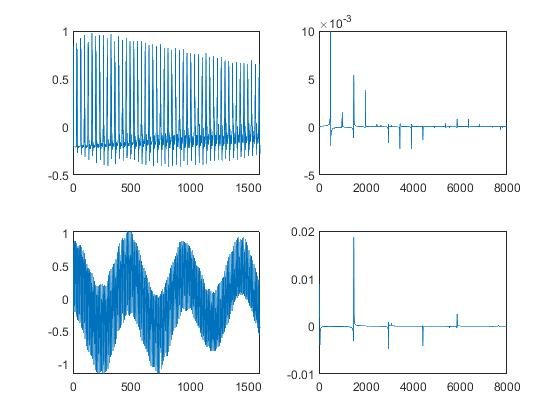
\includegraphics[width=13cm]{figura_vib_pos.jpg}
\end{figure}
 \medskip
\begin{figure}[!h]
\centering
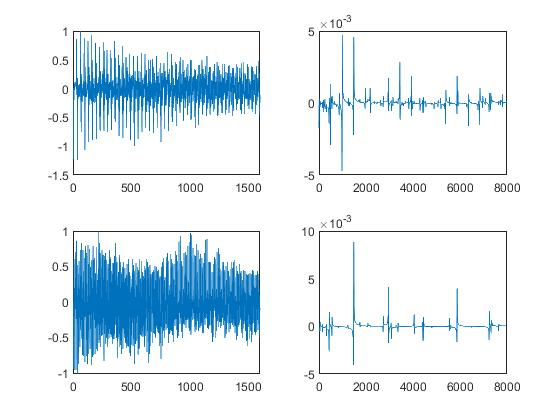
\includegraphics[width=13cm]{figura_vib_vel.jpg}
\end{figure}

\noindent
Dall'analisi delle frequenze nella seconda colonna osserviamo che nella prima corda la frequenza dominante è quella di circa $500Hz$, seguita dalle altre armoniche sue multiple: invece nella seconda cordalla frequenza dominante è di circa $1500Hz$, ovvero il triplo della prima armonica della prima corda. Questo è plausibilmente dovuto al fatto che le alte frequenze non risentono della oscillazione della massa grande, perciò sono quelle del tratto di corda teso tra il primo estremo e la massa grande, lungo circa un terzo della dell'intera corda, che spiega dunque il fattore 3.

Notiamo che l'analisi delle frequenze delle velocità rivela come le velocità della seconda corda siano molto più regolari rispetto a quelle della prima.



\end{document}